\begin{center}
    \begin{figure}[H]
        \centering

        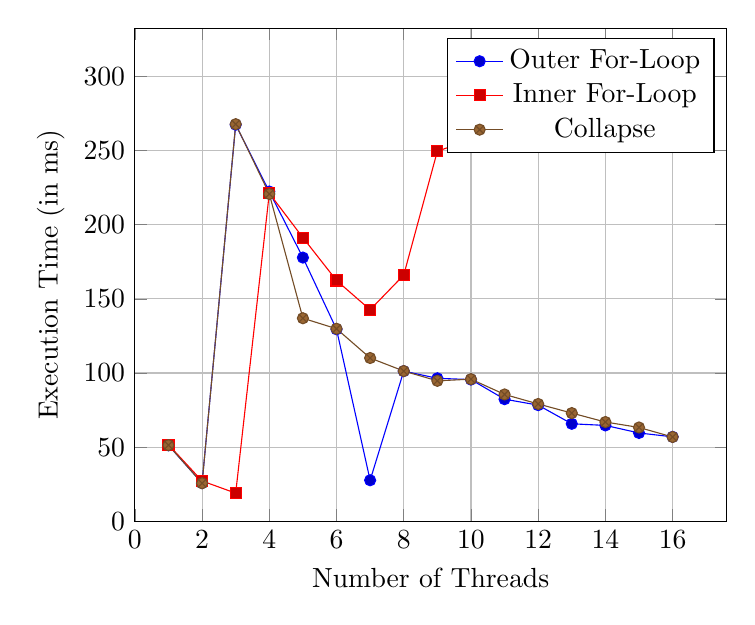
\begin{tikzpicture}
            \begin{axis}[
                title={},
                width=0.75\textwidth,
                xlabel={Number of Threads},
                ylabel={Execution Time (in ms)},
                xmin=0,
                ymin=0,
                grid=major
            ]
                \addplot coordinates {
                    (1,51.2614)(2,25.7889)(3,267.451)(4,222.391)(5,177.852)(6,129.484)(7,27.679)(8,101.276)(9,96.4451)(10,95.5812)(11,82.3594)(12,78.3406)(13,65.756)(14,64.6736)(15,59.5699)(16,56.9634)
                };
                \addlegendentry{Outer For-Loop}

                \addplot coordinates {
                    (1,51.6851)(2,27.2052)(3,18.9783)(4,221.218)(5,191.294)(6,162.421)(7,142.642)(8,166.08)(9,249.599)(10,257.363)(11,257.188)(12,258.531)(13,302.3)(14,289.604)(15,293.143)(16,293.078)
                };
                \addlegendentry{Inner For-Loop}       

                \addplot coordinates {
                    (1,51.3642)(2,25.6749)(3,267.826)(4,220.739)(5,136.95)(6,129.862)(7,110.125)(8,101.333)(9,94.7259)(10,95.8656)(11,85.5622)(12,79.1409)(13,72.9841)(14,66.952)(15,63.2878)(16,56.8636)
                };
                \addlegendentry{Collapse}
            \end{axis}
        \end{tikzpicture}
        \caption{HSV Performance Tests pnglogo-blk.png}
    \end{figure}
\end{center}